\section{Infrastructure}

The system proposed on this article follows the structure represented in the Fig. \ref{fig:infra_scheme}. As it has been introduced, it is composed by two blocks. The first one (\emph{perception} block) is responsible for performing the \emph{vision} tasks. Therefore, it determines, with the maximum possible precision, the position of every person found inside the image. It is here, as well, where it is discerned which of these persons is the one to be followed, in case it is seen. The second one (\emph{actuation} block) is designed to read and process that output from the previous block, and send suitable movement commands to the robot.\\



\begin{figure}[h]
	\centering
	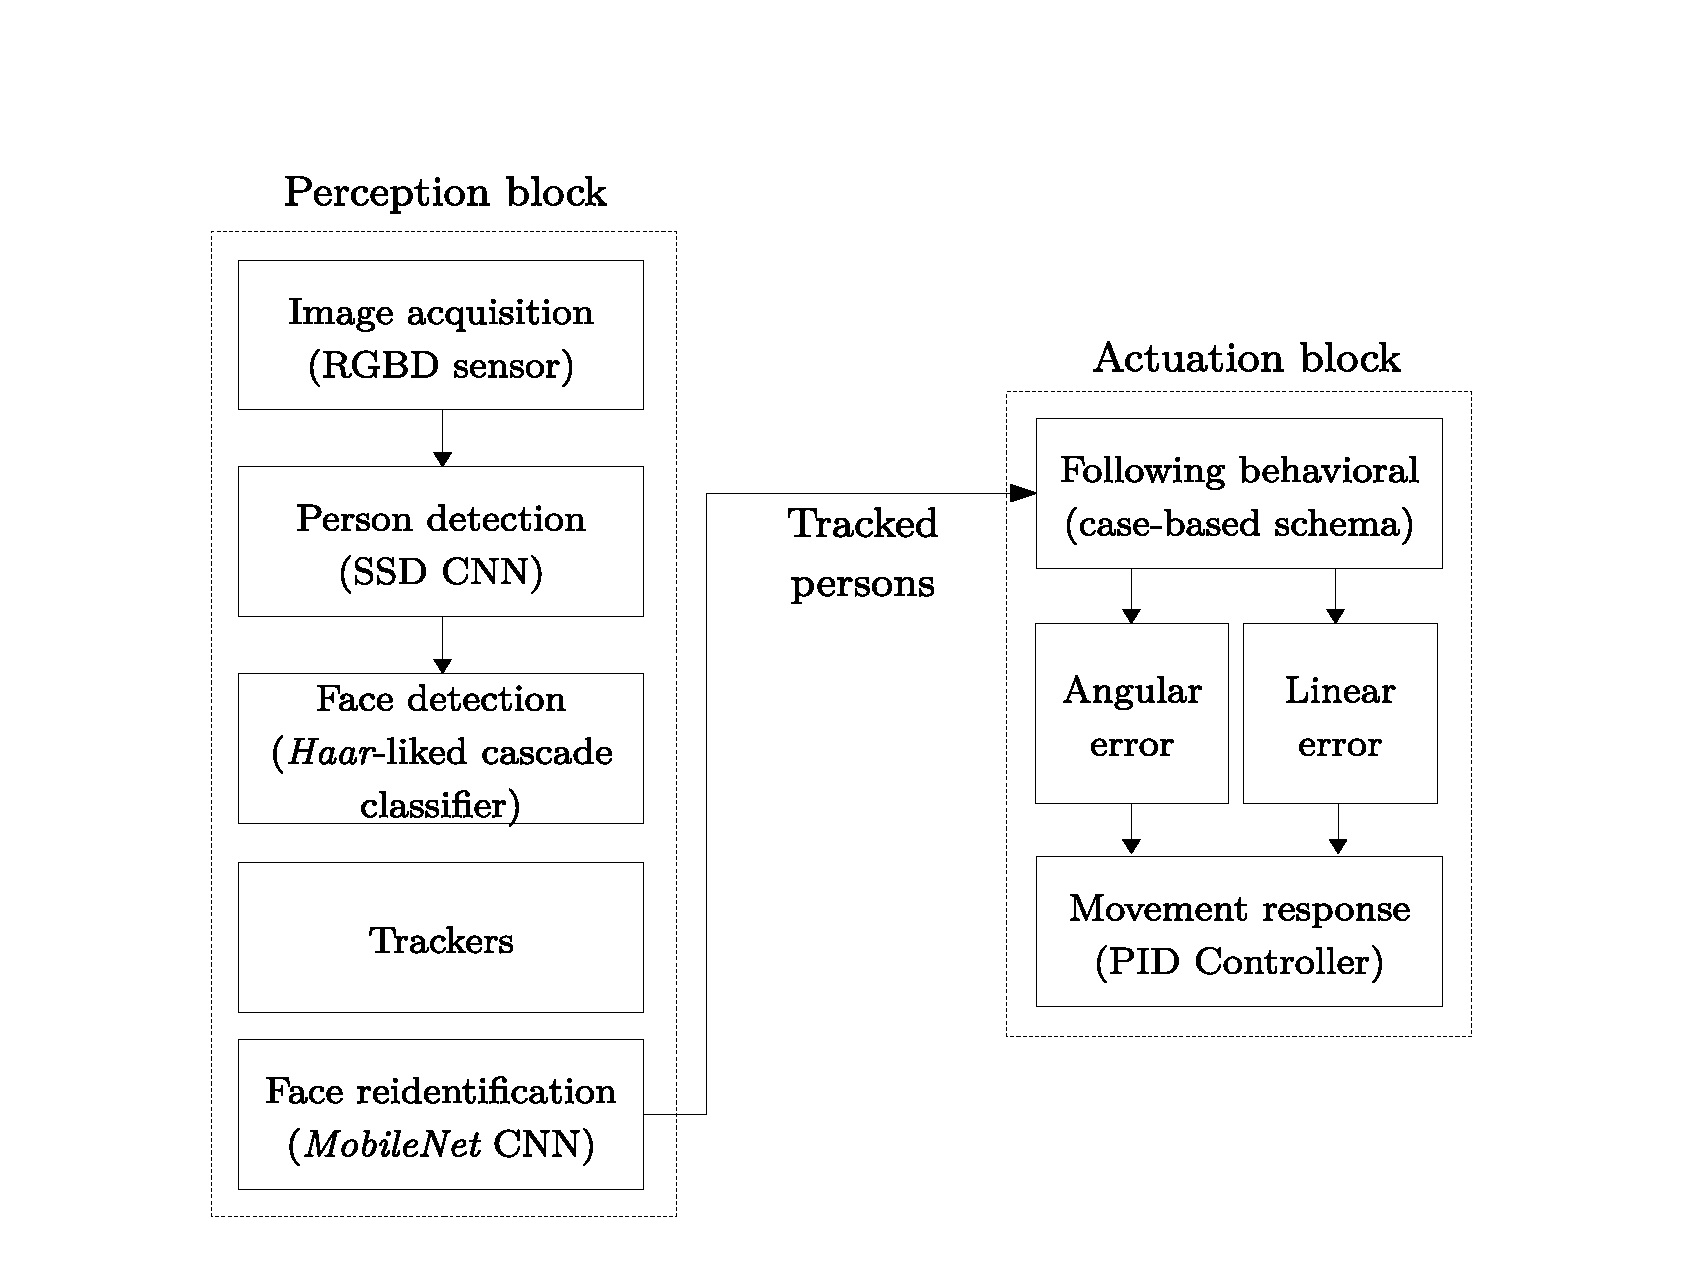
\includegraphics[width=3.2in]{images/system_schema}
	\caption{General structure of the proposed system.}
	\label{fig:infra_scheme}
\end{figure}



These mentioned blocks run on a computer, connected to both the RGBD sensor and the robot. The block processes are executed on a concurrent way, offering the advantage of a correct \emph{timing adaptation}. Hence, the system is designed to run properly on different hardware specifications on the base PC.